% Created by tikzDevice version 0.12.3.1 on 2023-03-27 19:33:31
% !TEX encoding = UTF-8 Unicode
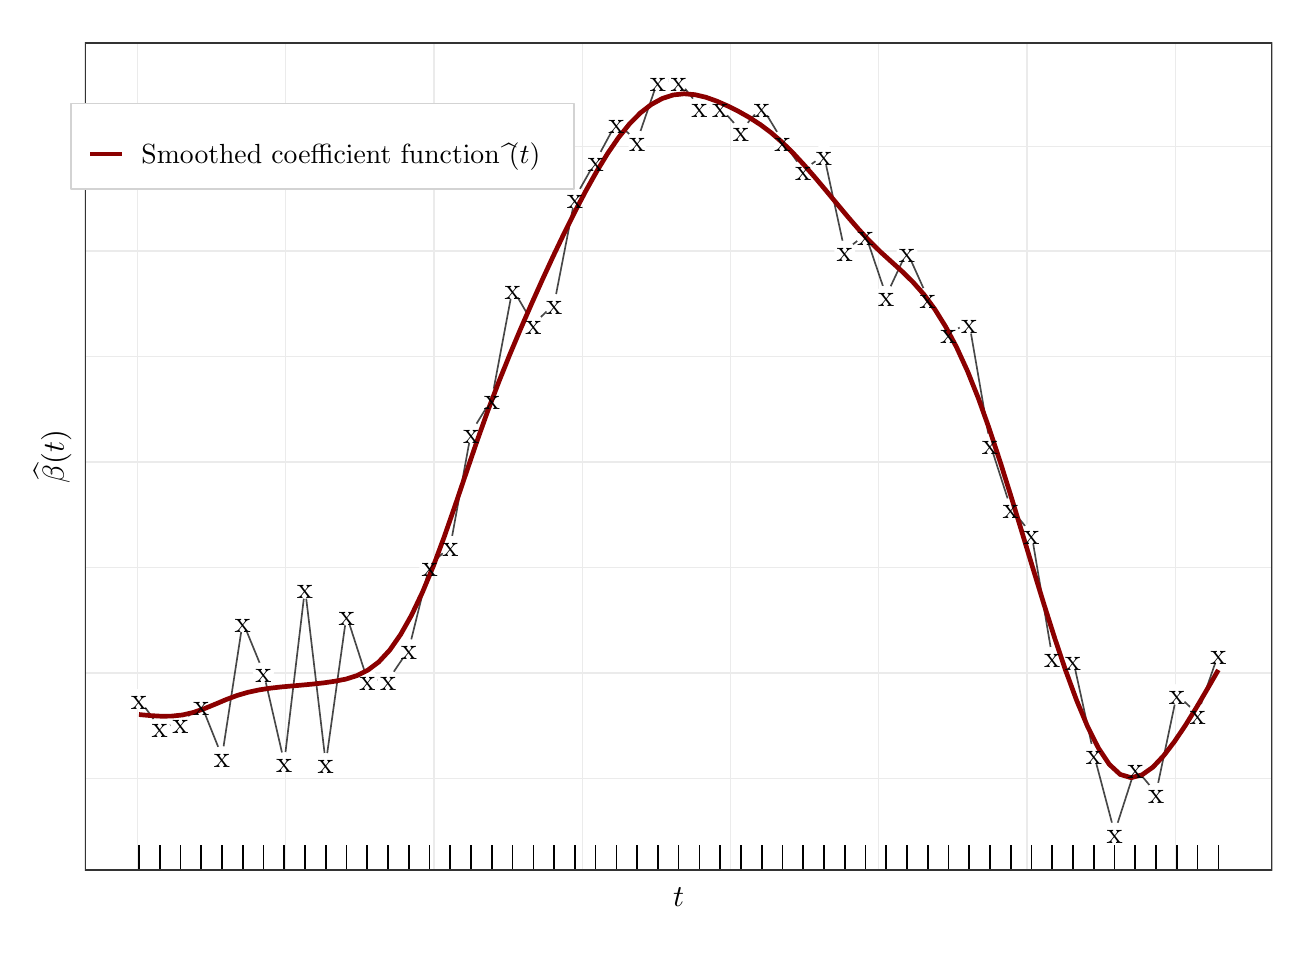
\begin{tikzpicture}[x=1pt,y=1pt]
\definecolor{fillColor}{RGB}{255,255,255}
\path[use as bounding box,fill=fillColor,fill opacity=0.00] (0,0) rectangle (455.24,325.17);
\begin{scope}
\path[clip] (  0.00,  0.00) rectangle (455.24,325.17);
\definecolor{drawColor}{RGB}{255,255,255}
\definecolor{fillColor}{RGB}{255,255,255}

\path[draw=drawColor,line width= 0.6pt,line join=round,line cap=round,fill=fillColor] (  0.00,  0.00) rectangle (455.24,325.17);
\end{scope}
\begin{scope}
\path[clip] ( 20.71, 20.71) rectangle (449.74,319.67);
\definecolor{fillColor}{RGB}{255,255,255}

\path[fill=fillColor] ( 20.71, 20.71) rectangle (449.74,319.67);
\definecolor{drawColor}{gray}{0.92}

\path[draw=drawColor,line width= 0.3pt,line join=round] ( 20.71, 54.00) --
	(449.74, 54.00);

\path[draw=drawColor,line width= 0.3pt,line join=round] ( 20.71,130.14) --
	(449.74,130.14);

\path[draw=drawColor,line width= 0.3pt,line join=round] ( 20.71,206.28) --
	(449.74,206.28);

\path[draw=drawColor,line width= 0.3pt,line join=round] ( 20.71,282.42) --
	(449.74,282.42);

\path[draw=drawColor,line width= 0.3pt,line join=round] ( 93.25, 20.71) --
	( 93.25,319.67);

\path[draw=drawColor,line width= 0.3pt,line join=round] (200.40, 20.71) --
	(200.40,319.67);

\path[draw=drawColor,line width= 0.3pt,line join=round] (307.56, 20.71) --
	(307.56,319.67);

\path[draw=drawColor,line width= 0.3pt,line join=round] (414.71, 20.71) --
	(414.71,319.67);

\path[draw=drawColor,line width= 0.6pt,line join=round] ( 20.71, 92.07) --
	(449.74, 92.07);

\path[draw=drawColor,line width= 0.6pt,line join=round] ( 20.71,168.21) --
	(449.74,168.21);

\path[draw=drawColor,line width= 0.6pt,line join=round] ( 20.71,244.35) --
	(449.74,244.35);

\path[draw=drawColor,line width= 0.6pt,line join=round] ( 39.68, 20.71) --
	( 39.68,319.67);

\path[draw=drawColor,line width= 0.6pt,line join=round] (146.83, 20.71) --
	(146.83,319.67);

\path[draw=drawColor,line width= 0.6pt,line join=round] (253.98, 20.71) --
	(253.98,319.67);

\path[draw=drawColor,line width= 0.6pt,line join=round] (361.13, 20.71) --
	(361.13,319.67);
\definecolor{drawColor}{RGB}{0,0,0}

\path[draw=drawColor,line width= 0.6pt,line join=round] ( 40.22, 20.71) -- ( 40.22, 29.68);

\path[draw=drawColor,line width= 0.6pt,line join=round] ( 47.72, 20.71) -- ( 47.72, 29.68);

\path[draw=drawColor,line width= 0.6pt,line join=round] ( 55.22, 20.71) -- ( 55.22, 29.68);

\path[draw=drawColor,line width= 0.6pt,line join=round] ( 62.72, 20.71) -- ( 62.72, 29.68);

\path[draw=drawColor,line width= 0.6pt,line join=round] ( 70.22, 20.71) -- ( 70.22, 29.68);

\path[draw=drawColor,line width= 0.6pt,line join=round] ( 77.72, 20.71) -- ( 77.72, 29.68);

\path[draw=drawColor,line width= 0.6pt,line join=round] ( 85.22, 20.71) -- ( 85.22, 29.68);

\path[draw=drawColor,line width= 0.6pt,line join=round] ( 92.72, 20.71) -- ( 92.72, 29.68);

\path[draw=drawColor,line width= 0.6pt,line join=round] (100.22, 20.71) -- (100.22, 29.68);

\path[draw=drawColor,line width= 0.6pt,line join=round] (107.72, 20.71) -- (107.72, 29.68);

\path[draw=drawColor,line width= 0.6pt,line join=round] (115.22, 20.71) -- (115.22, 29.68);

\path[draw=drawColor,line width= 0.6pt,line join=round] (122.72, 20.71) -- (122.72, 29.68);

\path[draw=drawColor,line width= 0.6pt,line join=round] (130.22, 20.71) -- (130.22, 29.68);

\path[draw=drawColor,line width= 0.6pt,line join=round] (137.72, 20.71) -- (137.72, 29.68);

\path[draw=drawColor,line width= 0.6pt,line join=round] (145.22, 20.71) -- (145.22, 29.68);

\path[draw=drawColor,line width= 0.6pt,line join=round] (152.72, 20.71) -- (152.72, 29.68);

\path[draw=drawColor,line width= 0.6pt,line join=round] (160.22, 20.71) -- (160.22, 29.68);

\path[draw=drawColor,line width= 0.6pt,line join=round] (167.72, 20.71) -- (167.72, 29.68);

\path[draw=drawColor,line width= 0.6pt,line join=round] (175.22, 20.71) -- (175.22, 29.68);

\path[draw=drawColor,line width= 0.6pt,line join=round] (182.73, 20.71) -- (182.73, 29.68);

\path[draw=drawColor,line width= 0.6pt,line join=round] (190.23, 20.71) -- (190.23, 29.68);

\path[draw=drawColor,line width= 0.6pt,line join=round] (197.73, 20.71) -- (197.73, 29.68);

\path[draw=drawColor,line width= 0.6pt,line join=round] (205.23, 20.71) -- (205.23, 29.68);

\path[draw=drawColor,line width= 0.6pt,line join=round] (212.73, 20.71) -- (212.73, 29.68);

\path[draw=drawColor,line width= 0.6pt,line join=round] (220.23, 20.71) -- (220.23, 29.68);

\path[draw=drawColor,line width= 0.6pt,line join=round] (227.73, 20.71) -- (227.73, 29.68);

\path[draw=drawColor,line width= 0.6pt,line join=round] (235.23, 20.71) -- (235.23, 29.68);

\path[draw=drawColor,line width= 0.6pt,line join=round] (242.73, 20.71) -- (242.73, 29.68);

\path[draw=drawColor,line width= 0.6pt,line join=round] (250.23, 20.71) -- (250.23, 29.68);

\path[draw=drawColor,line width= 0.6pt,line join=round] (257.73, 20.71) -- (257.73, 29.68);

\path[draw=drawColor,line width= 0.6pt,line join=round] (265.23, 20.71) -- (265.23, 29.68);

\path[draw=drawColor,line width= 0.6pt,line join=round] (272.73, 20.71) -- (272.73, 29.68);

\path[draw=drawColor,line width= 0.6pt,line join=round] (280.23, 20.71) -- (280.23, 29.68);

\path[draw=drawColor,line width= 0.6pt,line join=round] (287.73, 20.71) -- (287.73, 29.68);

\path[draw=drawColor,line width= 0.6pt,line join=round] (295.23, 20.71) -- (295.23, 29.68);

\path[draw=drawColor,line width= 0.6pt,line join=round] (302.73, 20.71) -- (302.73, 29.68);

\path[draw=drawColor,line width= 0.6pt,line join=round] (310.23, 20.71) -- (310.23, 29.68);

\path[draw=drawColor,line width= 0.6pt,line join=round] (317.73, 20.71) -- (317.73, 29.68);

\path[draw=drawColor,line width= 0.6pt,line join=round] (325.23, 20.71) -- (325.23, 29.68);

\path[draw=drawColor,line width= 0.6pt,line join=round] (332.74, 20.71) -- (332.74, 29.68);

\path[draw=drawColor,line width= 0.6pt,line join=round] (340.24, 20.71) -- (340.24, 29.68);

\path[draw=drawColor,line width= 0.6pt,line join=round] (347.74, 20.71) -- (347.74, 29.68);

\path[draw=drawColor,line width= 0.6pt,line join=round] (355.24, 20.71) -- (355.24, 29.68);

\path[draw=drawColor,line width= 0.6pt,line join=round] (362.74, 20.71) -- (362.74, 29.68);

\path[draw=drawColor,line width= 0.6pt,line join=round] (370.24, 20.71) -- (370.24, 29.68);

\path[draw=drawColor,line width= 0.6pt,line join=round] (377.74, 20.71) -- (377.74, 29.68);

\path[draw=drawColor,line width= 0.6pt,line join=round] (385.24, 20.71) -- (385.24, 29.68);

\path[draw=drawColor,line width= 0.6pt,line join=round] (392.74, 20.71) -- (392.74, 29.68);

\path[draw=drawColor,line width= 0.6pt,line join=round] (400.24, 20.71) -- (400.24, 29.68);

\path[draw=drawColor,line width= 0.6pt,line join=round] (407.74, 20.71) -- (407.74, 29.68);

\path[draw=drawColor,line width= 0.6pt,line join=round] (415.24, 20.71) -- (415.24, 29.68);

\path[draw=drawColor,line width= 0.6pt,line join=round] (422.74, 20.71) -- (422.74, 29.68);

\path[draw=drawColor,line width= 0.6pt,line join=round] (430.24, 20.71) -- (430.24, 29.68);
\definecolor{drawColor}{RGB}{10,10,10}

\path[draw=drawColor,draw opacity=0.75,line width= 0.6pt,line join=round] ( 40.22, 82.50) --
	( 47.72, 72.34) --
	( 55.22, 73.88) --
	( 62.72, 80.60) --
	( 70.22, 61.80) --
	( 77.72,110.49) --
	( 85.22, 92.20) --
	( 92.72, 59.66) --
	(100.22,122.55) --
	(107.72, 59.32) --
	(115.22,112.89) --
	(122.72, 89.58) --
	(130.22, 89.33) --
	(137.72,100.52) --
	(145.22,130.77) --
	(152.72,137.84) --
	(160.22,178.87) --
	(167.72,191.06) --
	(175.22,230.83) --
	(182.73,218.01) --
	(190.23,225.23) --
	(197.73,263.66) --
	(205.23,276.96) --
	(212.73,290.83) --
	(220.23,284.27) --
	(227.73,306.08) --
	(235.23,306.02) --
	(242.73,296.60) --
	(250.23,296.34) --
	(257.73,287.92) --
	(265.23,296.68) --
	(272.73,284.30) --
	(280.23,273.70) --
	(287.73,279.09) --
	(295.23,244.55) --
	(302.73,250.43) --
	(310.23,228.28) --
	(317.73,244.29) --
	(325.23,227.57) --
	(332.74,215.00) --
	(340.24,218.29) --
	(347.74,174.85) --
	(355.24,151.50) --
	(362.74,142.23) --
	(370.24, 97.66) --
	(377.74, 96.82) --
	(385.24, 62.69) --
	(392.74, 34.30) --
	(400.24, 57.59) --
	(407.74, 48.63) --
	(415.24, 84.22) --
	(422.74, 77.17) --
	(430.24, 98.81);
\definecolor{drawColor}{RGB}{255,255,255}

\path[draw=drawColor,line width= 0.4pt,line join=round,line cap=round,fill=fillColor] ( 40.22, 82.50) circle (  3.57);

\path[draw=drawColor,line width= 0.4pt,line join=round,line cap=round,fill=fillColor] ( 47.72, 72.34) circle (  3.57);

\path[draw=drawColor,line width= 0.4pt,line join=round,line cap=round,fill=fillColor] ( 55.22, 73.88) circle (  3.57);

\path[draw=drawColor,line width= 0.4pt,line join=round,line cap=round,fill=fillColor] ( 62.72, 80.60) circle (  3.57);

\path[draw=drawColor,line width= 0.4pt,line join=round,line cap=round,fill=fillColor] ( 70.22, 61.80) circle (  3.57);

\path[draw=drawColor,line width= 0.4pt,line join=round,line cap=round,fill=fillColor] ( 77.72,110.49) circle (  3.57);

\path[draw=drawColor,line width= 0.4pt,line join=round,line cap=round,fill=fillColor] ( 85.22, 92.20) circle (  3.57);

\path[draw=drawColor,line width= 0.4pt,line join=round,line cap=round,fill=fillColor] ( 92.72, 59.66) circle (  3.57);

\path[draw=drawColor,line width= 0.4pt,line join=round,line cap=round,fill=fillColor] (100.22,122.55) circle (  3.57);

\path[draw=drawColor,line width= 0.4pt,line join=round,line cap=round,fill=fillColor] (107.72, 59.32) circle (  3.57);

\path[draw=drawColor,line width= 0.4pt,line join=round,line cap=round,fill=fillColor] (115.22,112.89) circle (  3.57);

\path[draw=drawColor,line width= 0.4pt,line join=round,line cap=round,fill=fillColor] (122.72, 89.58) circle (  3.57);

\path[draw=drawColor,line width= 0.4pt,line join=round,line cap=round,fill=fillColor] (130.22, 89.33) circle (  3.57);

\path[draw=drawColor,line width= 0.4pt,line join=round,line cap=round,fill=fillColor] (137.72,100.52) circle (  3.57);

\path[draw=drawColor,line width= 0.4pt,line join=round,line cap=round,fill=fillColor] (145.22,130.77) circle (  3.57);

\path[draw=drawColor,line width= 0.4pt,line join=round,line cap=round,fill=fillColor] (152.72,137.84) circle (  3.57);

\path[draw=drawColor,line width= 0.4pt,line join=round,line cap=round,fill=fillColor] (160.22,178.87) circle (  3.57);

\path[draw=drawColor,line width= 0.4pt,line join=round,line cap=round,fill=fillColor] (167.72,191.06) circle (  3.57);

\path[draw=drawColor,line width= 0.4pt,line join=round,line cap=round,fill=fillColor] (175.22,230.83) circle (  3.57);

\path[draw=drawColor,line width= 0.4pt,line join=round,line cap=round,fill=fillColor] (182.73,218.01) circle (  3.57);

\path[draw=drawColor,line width= 0.4pt,line join=round,line cap=round,fill=fillColor] (190.23,225.23) circle (  3.57);

\path[draw=drawColor,line width= 0.4pt,line join=round,line cap=round,fill=fillColor] (197.73,263.66) circle (  3.57);

\path[draw=drawColor,line width= 0.4pt,line join=round,line cap=round,fill=fillColor] (205.23,276.96) circle (  3.57);

\path[draw=drawColor,line width= 0.4pt,line join=round,line cap=round,fill=fillColor] (212.73,290.83) circle (  3.57);

\path[draw=drawColor,line width= 0.4pt,line join=round,line cap=round,fill=fillColor] (220.23,284.27) circle (  3.57);

\path[draw=drawColor,line width= 0.4pt,line join=round,line cap=round,fill=fillColor] (227.73,306.08) circle (  3.57);

\path[draw=drawColor,line width= 0.4pt,line join=round,line cap=round,fill=fillColor] (235.23,306.02) circle (  3.57);

\path[draw=drawColor,line width= 0.4pt,line join=round,line cap=round,fill=fillColor] (242.73,296.60) circle (  3.57);

\path[draw=drawColor,line width= 0.4pt,line join=round,line cap=round,fill=fillColor] (250.23,296.34) circle (  3.57);

\path[draw=drawColor,line width= 0.4pt,line join=round,line cap=round,fill=fillColor] (257.73,287.92) circle (  3.57);

\path[draw=drawColor,line width= 0.4pt,line join=round,line cap=round,fill=fillColor] (265.23,296.68) circle (  3.57);

\path[draw=drawColor,line width= 0.4pt,line join=round,line cap=round,fill=fillColor] (272.73,284.30) circle (  3.57);

\path[draw=drawColor,line width= 0.4pt,line join=round,line cap=round,fill=fillColor] (280.23,273.70) circle (  3.57);

\path[draw=drawColor,line width= 0.4pt,line join=round,line cap=round,fill=fillColor] (287.73,279.09) circle (  3.57);

\path[draw=drawColor,line width= 0.4pt,line join=round,line cap=round,fill=fillColor] (295.23,244.55) circle (  3.57);

\path[draw=drawColor,line width= 0.4pt,line join=round,line cap=round,fill=fillColor] (302.73,250.43) circle (  3.57);

\path[draw=drawColor,line width= 0.4pt,line join=round,line cap=round,fill=fillColor] (310.23,228.28) circle (  3.57);

\path[draw=drawColor,line width= 0.4pt,line join=round,line cap=round,fill=fillColor] (317.73,244.29) circle (  3.57);

\path[draw=drawColor,line width= 0.4pt,line join=round,line cap=round,fill=fillColor] (325.23,227.57) circle (  3.57);

\path[draw=drawColor,line width= 0.4pt,line join=round,line cap=round,fill=fillColor] (332.74,215.00) circle (  3.57);

\path[draw=drawColor,line width= 0.4pt,line join=round,line cap=round,fill=fillColor] (340.24,218.29) circle (  3.57);

\path[draw=drawColor,line width= 0.4pt,line join=round,line cap=round,fill=fillColor] (347.74,174.85) circle (  3.57);

\path[draw=drawColor,line width= 0.4pt,line join=round,line cap=round,fill=fillColor] (355.24,151.50) circle (  3.57);

\path[draw=drawColor,line width= 0.4pt,line join=round,line cap=round,fill=fillColor] (362.74,142.23) circle (  3.57);

\path[draw=drawColor,line width= 0.4pt,line join=round,line cap=round,fill=fillColor] (370.24, 97.66) circle (  3.57);

\path[draw=drawColor,line width= 0.4pt,line join=round,line cap=round,fill=fillColor] (377.74, 96.82) circle (  3.57);

\path[draw=drawColor,line width= 0.4pt,line join=round,line cap=round,fill=fillColor] (385.24, 62.69) circle (  3.57);

\path[draw=drawColor,line width= 0.4pt,line join=round,line cap=round,fill=fillColor] (392.74, 34.30) circle (  3.57);

\path[draw=drawColor,line width= 0.4pt,line join=round,line cap=round,fill=fillColor] (400.24, 57.59) circle (  3.57);

\path[draw=drawColor,line width= 0.4pt,line join=round,line cap=round,fill=fillColor] (407.74, 48.63) circle (  3.57);

\path[draw=drawColor,line width= 0.4pt,line join=round,line cap=round,fill=fillColor] (415.24, 84.22) circle (  3.57);

\path[draw=drawColor,line width= 0.4pt,line join=round,line cap=round,fill=fillColor] (422.74, 77.17) circle (  3.57);

\path[draw=drawColor,line width= 0.4pt,line join=round,line cap=round,fill=fillColor] (430.24, 98.81) circle (  3.57);
\definecolor{drawColor}{RGB}{139,0,0}

\path[draw=drawColor,line width= 1.7pt,line join=round] ( 40.22, 76.97) --
	( 44.16, 76.60) --
	( 48.09, 76.37) --
	( 52.03, 76.40) --
	( 55.97, 76.82) --
	( 59.91, 77.73) --
	( 63.85, 79.10) --
	( 67.79, 80.72) --
	( 71.73, 82.38) --
	( 75.67, 83.86) --
	( 79.61, 85.01) --
	( 83.55, 85.86) --
	( 87.49, 86.47) --
	( 91.43, 86.92) --
	( 95.37, 87.28) --
	( 99.31, 87.63) --
	(103.25, 88.00) --
	(107.19, 88.44) --
	(111.13, 89.02) --
	(115.07, 89.80) --
	(119.01, 91.05) --
	(122.95, 93.02) --
	(126.89, 96.00) --
	(130.83,100.25) --
	(134.77,105.90) --
	(138.71,112.88) --
	(142.65,121.14) --
	(146.59,130.62) --
	(150.53,141.21) --
	(154.47,152.54) --
	(158.41,164.19) --
	(162.35,175.74) --
	(166.28,186.77) --
	(170.22,197.13) --
	(174.16,206.92) --
	(178.10,216.28) --
	(182.04,225.31) --
	(185.98,234.10) --
	(189.92,242.64) --
	(193.86,250.88) --
	(197.80,258.79) --
	(201.74,266.30) --
	(205.68,273.34) --
	(209.62,279.80) --
	(213.56,285.53) --
	(217.50,290.43) --
	(221.44,294.40) --
	(225.38,297.44) --
	(229.32,299.58) --
	(233.26,300.85) --
	(237.20,301.28) --
	(241.14,300.95) --
	(245.08,300.02) --
	(249.02,298.61) --
	(252.96,296.87) --
	(256.90,294.90) --
	(260.84,292.67) --
	(264.78,290.11) --
	(268.72,287.15) --
	(272.66,283.72) --
	(276.60,279.84) --
	(280.53,275.59) --
	(284.47,271.08) --
	(288.41,266.39) --
	(292.35,261.63) --
	(296.29,256.91) --
	(300.23,252.35) --
	(304.17,248.08) --
	(308.11,244.20) --
	(312.05,240.63) --
	(315.99,237.07) --
	(319.93,233.20) --
	(323.87,228.73) --
	(327.81,223.39) --
	(331.75,217.05) --
	(335.69,209.61) --
	(339.63,201.01) --
	(343.57,191.14) --
	(347.51,180.11) --
	(351.45,168.18) --
	(355.39,155.62) --
	(359.33,142.70) --
	(363.27,129.70) --
	(367.21,116.87) --
	(371.15,104.48) --
	(375.09, 92.80) --
	(379.03, 82.10) --
	(382.97, 72.68) --
	(386.91, 64.85) --
	(390.85, 58.95) --
	(394.78, 55.32) --
	(398.72, 54.15) --
	(402.66, 55.16) --
	(406.60, 57.96) --
	(410.54, 62.15) --
	(414.48, 67.32) --
	(418.42, 73.19) --
	(422.36, 79.56) --
	(426.30, 86.26) --
	(430.24, 93.08);
\definecolor{drawColor}{RGB}{0,0,0}

\node[text=drawColor,anchor=base,inner sep=0pt, outer sep=0pt, scale=  1.10] at ( 40.22, 78.70) {x};

\node[text=drawColor,anchor=base,inner sep=0pt, outer sep=0pt, scale=  1.10] at ( 47.72, 68.54) {x};

\node[text=drawColor,anchor=base,inner sep=0pt, outer sep=0pt, scale=  1.10] at ( 55.22, 70.08) {x};

\node[text=drawColor,anchor=base,inner sep=0pt, outer sep=0pt, scale=  1.10] at ( 62.72, 76.79) {x};

\node[text=drawColor,anchor=base,inner sep=0pt, outer sep=0pt, scale=  1.10] at ( 70.22, 58.00) {x};

\node[text=drawColor,anchor=base,inner sep=0pt, outer sep=0pt, scale=  1.10] at ( 77.72,106.69) {x};

\node[text=drawColor,anchor=base,inner sep=0pt, outer sep=0pt, scale=  1.10] at ( 85.22, 88.40) {x};

\node[text=drawColor,anchor=base,inner sep=0pt, outer sep=0pt, scale=  1.10] at ( 92.72, 55.86) {x};

\node[text=drawColor,anchor=base,inner sep=0pt, outer sep=0pt, scale=  1.10] at (100.22,118.75) {x};

\node[text=drawColor,anchor=base,inner sep=0pt, outer sep=0pt, scale=  1.10] at (107.72, 55.51) {x};

\node[text=drawColor,anchor=base,inner sep=0pt, outer sep=0pt, scale=  1.10] at (115.22,109.09) {x};

\node[text=drawColor,anchor=base,inner sep=0pt, outer sep=0pt, scale=  1.10] at (122.72, 85.78) {x};

\node[text=drawColor,anchor=base,inner sep=0pt, outer sep=0pt, scale=  1.10] at (130.22, 85.53) {x};

\node[text=drawColor,anchor=base,inner sep=0pt, outer sep=0pt, scale=  1.10] at (137.72, 96.72) {x};

\node[text=drawColor,anchor=base,inner sep=0pt, outer sep=0pt, scale=  1.10] at (145.22,126.97) {x};

\node[text=drawColor,anchor=base,inner sep=0pt, outer sep=0pt, scale=  1.10] at (152.72,134.04) {x};

\node[text=drawColor,anchor=base,inner sep=0pt, outer sep=0pt, scale=  1.10] at (160.22,175.07) {x};

\node[text=drawColor,anchor=base,inner sep=0pt, outer sep=0pt, scale=  1.10] at (167.72,187.26) {x};

\node[text=drawColor,anchor=base,inner sep=0pt, outer sep=0pt, scale=  1.10] at (175.22,227.03) {x};

\node[text=drawColor,anchor=base,inner sep=0pt, outer sep=0pt, scale=  1.10] at (182.73,214.21) {x};

\node[text=drawColor,anchor=base,inner sep=0pt, outer sep=0pt, scale=  1.10] at (190.23,221.43) {x};

\node[text=drawColor,anchor=base,inner sep=0pt, outer sep=0pt, scale=  1.10] at (197.73,259.86) {x};

\node[text=drawColor,anchor=base,inner sep=0pt, outer sep=0pt, scale=  1.10] at (205.23,273.16) {x};

\node[text=drawColor,anchor=base,inner sep=0pt, outer sep=0pt, scale=  1.10] at (212.73,287.03) {x};

\node[text=drawColor,anchor=base,inner sep=0pt, outer sep=0pt, scale=  1.10] at (220.23,280.47) {x};

\node[text=drawColor,anchor=base,inner sep=0pt, outer sep=0pt, scale=  1.10] at (227.73,302.28) {x};

\node[text=drawColor,anchor=base,inner sep=0pt, outer sep=0pt, scale=  1.10] at (235.23,302.22) {x};

\node[text=drawColor,anchor=base,inner sep=0pt, outer sep=0pt, scale=  1.10] at (242.73,292.80) {x};

\node[text=drawColor,anchor=base,inner sep=0pt, outer sep=0pt, scale=  1.10] at (250.23,292.54) {x};

\node[text=drawColor,anchor=base,inner sep=0pt, outer sep=0pt, scale=  1.10] at (257.73,284.12) {x};

\node[text=drawColor,anchor=base,inner sep=0pt, outer sep=0pt, scale=  1.10] at (265.23,292.88) {x};

\node[text=drawColor,anchor=base,inner sep=0pt, outer sep=0pt, scale=  1.10] at (272.73,280.50) {x};

\node[text=drawColor,anchor=base,inner sep=0pt, outer sep=0pt, scale=  1.10] at (280.23,269.89) {x};

\node[text=drawColor,anchor=base,inner sep=0pt, outer sep=0pt, scale=  1.10] at (287.73,275.29) {x};

\node[text=drawColor,anchor=base,inner sep=0pt, outer sep=0pt, scale=  1.10] at (295.23,240.75) {x};

\node[text=drawColor,anchor=base,inner sep=0pt, outer sep=0pt, scale=  1.10] at (302.73,246.63) {x};

\node[text=drawColor,anchor=base,inner sep=0pt, outer sep=0pt, scale=  1.10] at (310.23,224.48) {x};

\node[text=drawColor,anchor=base,inner sep=0pt, outer sep=0pt, scale=  1.10] at (317.73,240.49) {x};

\node[text=drawColor,anchor=base,inner sep=0pt, outer sep=0pt, scale=  1.10] at (325.23,223.77) {x};

\node[text=drawColor,anchor=base,inner sep=0pt, outer sep=0pt, scale=  1.10] at (332.74,211.20) {x};

\node[text=drawColor,anchor=base,inner sep=0pt, outer sep=0pt, scale=  1.10] at (340.24,214.49) {x};

\node[text=drawColor,anchor=base,inner sep=0pt, outer sep=0pt, scale=  1.10] at (347.74,171.05) {x};

\node[text=drawColor,anchor=base,inner sep=0pt, outer sep=0pt, scale=  1.10] at (355.24,147.70) {x};

\node[text=drawColor,anchor=base,inner sep=0pt, outer sep=0pt, scale=  1.10] at (362.74,138.42) {x};

\node[text=drawColor,anchor=base,inner sep=0pt, outer sep=0pt, scale=  1.10] at (370.24, 93.85) {x};

\node[text=drawColor,anchor=base,inner sep=0pt, outer sep=0pt, scale=  1.10] at (377.74, 93.02) {x};

\node[text=drawColor,anchor=base,inner sep=0pt, outer sep=0pt, scale=  1.10] at (385.24, 58.89) {x};

\node[text=drawColor,anchor=base,inner sep=0pt, outer sep=0pt, scale=  1.10] at (392.74, 30.50) {x};

\node[text=drawColor,anchor=base,inner sep=0pt, outer sep=0pt, scale=  1.10] at (400.24, 53.79) {x};

\node[text=drawColor,anchor=base,inner sep=0pt, outer sep=0pt, scale=  1.10] at (407.74, 44.83) {x};

\node[text=drawColor,anchor=base,inner sep=0pt, outer sep=0pt, scale=  1.10] at (415.24, 80.42) {x};

\node[text=drawColor,anchor=base,inner sep=0pt, outer sep=0pt, scale=  1.10] at (422.74, 73.37) {x};

\node[text=drawColor,anchor=base,inner sep=0pt, outer sep=0pt, scale=  1.10] at (430.24, 95.01) {x};
\definecolor{drawColor}{gray}{0.20}

\path[draw=drawColor,line width= 0.6pt,line join=round,line cap=round] ( 20.71, 20.71) rectangle (449.74,319.67);
\end{scope}
\begin{scope}
\path[clip] (  0.00,  0.00) rectangle (455.24,325.17);
\definecolor{drawColor}{RGB}{0,0,0}

\node[text=drawColor,anchor=base,inner sep=0pt, outer sep=0pt, scale=  1.10] at (235.23,  7.64) {$t$};
\end{scope}
\begin{scope}
\path[clip] (  0.00,  0.00) rectangle (455.24,325.17);
\definecolor{drawColor}{RGB}{0,0,0}

\node[text=drawColor,rotate= 90.00,anchor=base,inner sep=0pt, outer sep=0pt, scale=  1.10] at ( 13.08,170.19) {$\widehat{\beta} (t)$};
\end{scope}
\begin{scope}
\path[clip] (  0.00,  0.00) rectangle (455.24,325.17);
\definecolor{drawColor}{RGB}{211,211,211}
\definecolor{fillColor}{RGB}{255,255,255}

\path[draw=drawColor,line width= 0.6pt,line join=round,line cap=round,fill=fillColor] ( 15.66,266.83) rectangle (197.38,297.78);
\end{scope}
\begin{scope}
\path[clip] (  0.00,  0.00) rectangle (455.24,325.17);
\definecolor{fillColor}{RGB}{255,255,255}

\path[fill=fillColor] ( 21.16,272.33) rectangle ( 35.62,286.78);
\end{scope}
\begin{scope}
\path[clip] (  0.00,  0.00) rectangle (455.24,325.17);
\definecolor{drawColor}{RGB}{139,0,0}

\path[draw=drawColor,line width= 1.7pt,line join=round] ( 22.61,279.55) -- ( 34.17,279.55);
\end{scope}
\begin{scope}
\path[clip] (  0.00,  0.00) rectangle (455.24,325.17);
\definecolor{drawColor}{RGB}{0,0,0}

\node[text=drawColor,anchor=base west,inner sep=0pt, outer sep=0pt, scale=  1.00] at ( 41.12,276.11) {Smoothed coefficient function $\widehat{\upbeta} (t)$};
\end{scope}
\end{tikzpicture}
